\documentclass[twoside]{book}

% Packages required by doxygen
\usepackage{fixltx2e}
\usepackage{calc}
\usepackage{doxygen}
\usepackage[export]{adjustbox} % also loads graphicx
\usepackage{graphicx}
\usepackage[utf8]{inputenc}
\usepackage{makeidx}
\usepackage{multicol}
\usepackage{multirow}
\PassOptionsToPackage{warn}{textcomp}
\usepackage{textcomp}
\usepackage[nointegrals]{wasysym}
\usepackage[table]{xcolor}

% Font selection
\usepackage[T1]{fontenc}
\usepackage[scaled=.90]{helvet}
\usepackage{courier}
\usepackage{amssymb}
\usepackage{sectsty}
\renewcommand{\familydefault}{\sfdefault}
\allsectionsfont{%
  \fontseries{bc}\selectfont%
  \color{darkgray}%
}
\renewcommand{\DoxyLabelFont}{%
  \fontseries{bc}\selectfont%
  \color{darkgray}%
}
\newcommand{\+}{\discretionary{\mbox{\scriptsize$\hookleftarrow$}}{}{}}

% Page & text layout
\usepackage{geometry}
\geometry{%
  a4paper,%
  top=2.5cm,%
  bottom=2.5cm,%
  left=2.5cm,%
  right=2.5cm%
}
\tolerance=750
\hfuzz=15pt
\hbadness=750
\setlength{\emergencystretch}{15pt}
\setlength{\parindent}{0cm}
\setlength{\parskip}{3ex plus 2ex minus 2ex}
\makeatletter
\renewcommand{\paragraph}{%
  \@startsection{paragraph}{4}{0ex}{-1.0ex}{1.0ex}{%
    \normalfont\normalsize\bfseries\SS@parafont%
  }%
}
\renewcommand{\subparagraph}{%
  \@startsection{subparagraph}{5}{0ex}{-1.0ex}{1.0ex}{%
    \normalfont\normalsize\bfseries\SS@subparafont%
  }%
}
\makeatother

% Headers & footers
\usepackage{fancyhdr}
\pagestyle{fancyplain}
\fancyhead[LE]{\fancyplain{}{\bfseries\thepage}}
\fancyhead[CE]{\fancyplain{}{}}
\fancyhead[RE]{\fancyplain{}{\bfseries\leftmark}}
\fancyhead[LO]{\fancyplain{}{\bfseries\rightmark}}
\fancyhead[CO]{\fancyplain{}{}}
\fancyhead[RO]{\fancyplain{}{\bfseries\thepage}}
\fancyfoot[LE]{\fancyplain{}{}}
\fancyfoot[CE]{\fancyplain{}{}}
\fancyfoot[RE]{\fancyplain{}{\bfseries\scriptsize Generated by Doxygen }}
\fancyfoot[LO]{\fancyplain{}{\bfseries\scriptsize Generated by Doxygen }}
\fancyfoot[CO]{\fancyplain{}{}}
\fancyfoot[RO]{\fancyplain{}{}}
\renewcommand{\footrulewidth}{0.4pt}
\renewcommand{\chaptermark}[1]{%
  \markboth{#1}{}%
}
\renewcommand{\sectionmark}[1]{%
  \markright{\thesection\ #1}%
}

% Indices & bibliography
\usepackage{natbib}
\usepackage[titles]{tocloft}
\setcounter{tocdepth}{3}
\setcounter{secnumdepth}{5}
\makeindex

% Hyperlinks (required, but should be loaded last)
\usepackage{ifpdf}
\ifpdf
  \usepackage[pdftex,pagebackref=true]{hyperref}
\else
  \usepackage[ps2pdf,pagebackref=true]{hyperref}
\fi
\hypersetup{%
  colorlinks=true,%
  linkcolor=blue,%
  citecolor=blue,%
  unicode%
}

% Custom commands
\newcommand{\clearemptydoublepage}{%
  \newpage{\pagestyle{empty}\cleardoublepage}%
}

\usepackage{caption}
\captionsetup{labelsep=space,justification=centering,font={bf},singlelinecheck=off,skip=4pt,position=top}

%===== C O N T E N T S =====

\begin{document}

% Titlepage & ToC
\hypersetup{pageanchor=false,
             bookmarksnumbered=true,
             pdfencoding=unicode
            }
\pagenumbering{alph}
\begin{titlepage}
\vspace*{7cm}
\begin{center}%
{\Large My Project }\\
\vspace*{1cm}
{\large Generated by Doxygen 1.8.13}\\
\end{center}
\end{titlepage}
\clearemptydoublepage
\pagenumbering{roman}
\tableofcontents
\clearemptydoublepage
\pagenumbering{arabic}
\hypersetup{pageanchor=true}

%--- Begin generated contents ---
\chapter{Hierarchical Index}
\section{Class Hierarchy}
This inheritance list is sorted roughly, but not completely, alphabetically\+:\begin{DoxyCompactList}
\item P\+Applet\begin{DoxyCompactList}
\item \contentsline{section}{starlings}{\pageref{classstarlings}}{}
\end{DoxyCompactList}
\end{DoxyCompactList}

\chapter{Class Index}
\section{Class List}
Here are the classes, structs, unions and interfaces with brief descriptions\+:\begin{DoxyCompactList}
\item\contentsline{section}{\hyperlink{classstarlings}{starlings} }{\pageref{classstarlings}}{}
\end{DoxyCompactList}

\chapter{Class Documentation}
\hypertarget{classstarlings}{}\section{starlings Class Reference}
\label{classstarlings}\index{starlings@{starlings}}


Inheritance diagram for starlings\+:
\nopagebreak
\begin{figure}[H]
\begin{center}
\leavevmode
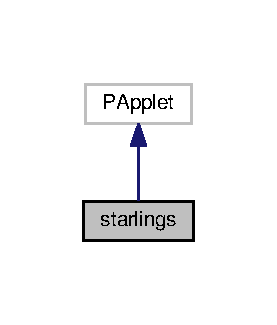
\includegraphics[width=133pt]{classstarlings__inherit__graph}
\end{center}
\end{figure}


Collaboration diagram for starlings\+:
\nopagebreak
\begin{figure}[H]
\begin{center}
\leavevmode
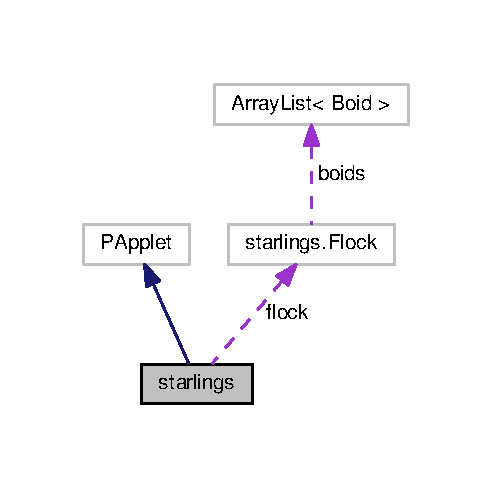
\includegraphics[width=236pt]{classstarlings__coll__graph}
\end{center}
\end{figure}
\subsection*{Classes}
\begin{DoxyCompactItemize}
\item 
class {\bfseries Boid}
\item 
class {\bfseries Flock}
\end{DoxyCompactItemize}
\subsection*{Public Member Functions}
\begin{DoxyCompactItemize}
\item 
void \hyperlink{classstarlings_ae3237d3011a7d17127f7c5d3b7db4c8d}{setup} ()
\item 
void \hyperlink{classstarlings_ab9dc1bf7e725edf0e21387669aaa38bc}{draw} ()
\item 
void \hyperlink{classstarlings_a7482acd0c545833aacce135b5a8bd573}{mouse\+Pressed} ()
\item 
\mbox{\Hypertarget{classstarlings_ab4389babbb4fcc756571ddb2a9f91cb9}\label{classstarlings_ab4389babbb4fcc756571ddb2a9f91cb9}} 
void {\bfseries settings} ()
\end{DoxyCompactItemize}
\subsection*{Static Public Member Functions}
\begin{DoxyCompactItemize}
\item 
\mbox{\Hypertarget{classstarlings_aacba2310e0f458e0429fa02404d137dc}\label{classstarlings_aacba2310e0f458e0429fa02404d137dc}} 
static void {\bfseries main} (String\mbox{[}$\,$\mbox{]} passed\+Args)
\end{DoxyCompactItemize}


\subsection{Member Function Documentation}
\mbox{\Hypertarget{classstarlings_ab9dc1bf7e725edf0e21387669aaa38bc}\label{classstarlings_ab9dc1bf7e725edf0e21387669aaa38bc}} 
\index{starlings@{starlings}!draw@{draw}}
\index{draw@{draw}!starlings@{starlings}}
\subsubsection{\texorpdfstring{draw()}{draw()}}
{\footnotesize\ttfamily void starlings.\+draw (\begin{DoxyParamCaption}{ }\end{DoxyParamCaption})\hspace{0.3cm}{\ttfamily [inline]}}

Renders the display on the screen\mbox{\Hypertarget{classstarlings_a7482acd0c545833aacce135b5a8bd573}\label{classstarlings_a7482acd0c545833aacce135b5a8bd573}} 
\index{starlings@{starlings}!mouse\+Pressed@{mouse\+Pressed}}
\index{mouse\+Pressed@{mouse\+Pressed}!starlings@{starlings}}
\subsubsection{\texorpdfstring{mouse\+Pressed()}{mousePressed()}}
{\footnotesize\ttfamily void starlings.\+mouse\+Pressed (\begin{DoxyParamCaption}{ }\end{DoxyParamCaption})\hspace{0.3cm}{\ttfamily [inline]}}

Adds new boids when detects a mouse click\mbox{\Hypertarget{classstarlings_ae3237d3011a7d17127f7c5d3b7db4c8d}\label{classstarlings_ae3237d3011a7d17127f7c5d3b7db4c8d}} 
\index{starlings@{starlings}!setup@{setup}}
\index{setup@{setup}!starlings@{starlings}}
\subsubsection{\texorpdfstring{setup()}{setup()}}
{\footnotesize\ttfamily void starlings.\+setup (\begin{DoxyParamCaption}{ }\end{DoxyParamCaption})\hspace{0.3cm}{\ttfamily [inline]}}

Is called to start the project Creates new Boids and starts the project

The documentation for this class was generated from the following file\+:\begin{DoxyCompactItemize}
\item 
documentation\+\_\+starlings.\+java\end{DoxyCompactItemize}

%--- End generated contents ---

% Index
\backmatter
\newpage
\phantomsection
\clearemptydoublepage
\addcontentsline{toc}{chapter}{Index}
\printindex

\end{document}
